% -*- Mode:TeX -*-

%% IMPORTANT: The official thesis specifications are available at:
%%            http://libraries.mit.edu/archives/thesis-specs/
%%
%%            Please verify your thesis' formatting and copyright
%%            assignment before submission.  If you notice any
%%            discrepancies between these templates and the 
%%            MIT Libraries' specs, please let us know
%%            by e-mailing thesis@mit.edu

%% The documentclass options along with the pagestyle can be used to generate
%% a technical report, a draft copy, or a regular thesis.  You may need to
%% re-specify the pagestyle after you \include  cover.tex.  For more
%% information, see the first few lines of mitthesis.cls. 

%\documentclass[12pt,vi,twoside]{mitthesis}
%%
%%  If you want your thesis copyright to you instead of MIT, use the
%%  ``vi'' option, as above.
%%
%\documentclass[12pt,twoside,leftblank]{mitthesis}
%%
%% If you want blank pages before new chapters to be labelled ``This
%% Page Intentionally Left Blank'', use the ``leftblank'' option, as
%% above. 

\documentclass[12pt,vi,twoside,singlespace]{mitthesis}
\usepackage{lgrind}
%% These have been added at the request of the MIT Libraries, because
%% some PDF conversions mess up the ligatures.  -LB, 1/22/2014
\usepackage{cmap}
\usepackage[T1]{fontenc}
\usepackage{amsmath}
\usepackage{amsthm}
\usepackage{amssymb}
\usepackage{amsfonts}
\usepackage{graphicx}
\usepackage{ftnxtra}
\usepackage{multirow}
\usepackage{mathcomp}
\usepackage{subcaption}
\usepackage[super]{nth}
\usepackage{hyperref}
\usepackage{bm}
\hypersetup{
    colorlinks=true,
    linkcolor=blue,
    citecolor = red,
}
\urlstyle{same}
\graphicspath{ {images/} }
\newcommand{\rnum}[1]{\uppercase\expandafter{\romannumeral #1\relax}}
\newcommand{\matr}[1]{\bm{#1}}
\pagestyle{headings}
%% This bit allows you to either specify only the files which you wish to
%% process, or `all' to process all files which you \include.
%% Krishna Sethuraman (1990).

\typein [\files]{Enter file names to process, (chap1,chap2 ...), or `all' to
process all files:}
\def\all{all}
\ifx\files\all \typeout{Including all files.} \else \typeout{Including only \files.} \includeonly{\files} \fi

%\makeatletter
%\renewcommand{\@biblabel}[1]{[#1]\hfill}
%\makeatother
\theoremstyle{definition}
\newtheorem{defn}{Definition}
\newtheorem{theorem}{Theorem}

\begin{document}
% -*-latex-*-
% 
% For questions, comments, concerns or complaints:
% thesis@mit.edu
% 
%
% $Log: cover.tex,v $
% Revision 1.8  2008/05/13 15:02:15  jdreed
% Degree month is June, not May.  Added note about prevdegrees.
% Arthur Smith's title updated
%
% Revision 1.7  2001/02/08 18:53:16  boojum
% changed some \newpages to \cleardoublepages
%
% Revision 1.6  1999/10/21 14:49:31  boojum
% changed comment referring to documentstyle
%
% Revision 1.5  1999/10/21 14:39:04  boojum
% *** empty log message ***
%
% Revision 1.4  1997/04/18  17:54:10  othomas
% added page numbers on abstract and cover, and made 1 abstract
% page the default rather than 2.  (anne hunter tells me this
% is the new institute standard.)
%
% Revision 1.4  1997/04/18  17:54:10  othomas
% added page numbers on abstract and cover, and made 1 abstract
% page the default rather than 2.  (anne hunter tells me this
% is the new institute standard.)
%
% Revision 1.3  93/05/17  17:06:29  starflt
% Added acknowledgements section (suggested by tompalka)
% 
% Revision 1.2  92/04/22  13:13:13  epeisach
% Fixes for 1991 course 6 requirements
% Phrase "and to grant others the right to do so" has been added to 
% permission clause
% Second copy of abstract is not counted as separate pages so numbering works
% out
% 
% Revision 1.1  92/04/22  13:08:20  epeisach

% NOTE:
% These templates make an effort to conform to the MIT Thesis specifications,
% however the specifications can change.  We recommend that you verify the
% layout of your title page with your thesis advisor and/or the MIT 
% Libraries before printing your final copy.
%\title{SCE16-0446\\
% Time-Dependent Shortest Path Queries on Mobile Devices}
\title{March Machine Learning Mania 2016 \\
Predict the 2016 NCAA Basketball Tournament}


\author{\begin{tabular}{ l l l}
Joe Tan Chin Yong & Data Scientist& U1521434C \\
Liu Zeyan & Data Analyst & U1421784C \\ 
Wei Yumou & Data Scientist & U1320554F \\ 
Xie Dai  & Statistician& U1340229K\\
\end{tabular}}
% If you wish to list your previous degrees on the cover page, use the 
% previous degrees command:
%       \prevdegrees{A.A., Harvard University (1985)}
% You can use the \\ command to list multiple previous degrees
%       \prevdegrees{B.S., University of California (1978) \\
%                    S.M., Massachusetts Institute of Technology (1981)}

\department{School of Computer Science and Engineering}

% If the thesis is for two degrees simultaneously, list them both
% separated by \and like this:
% \degree{Doctor of Philosophy \and Master of Science}
\degree{CE/CZ 4041 Machine Learning}

% As of the 2007-08 academic year, valid degree months are September, 
% February, or June.  The default is June.
\degreemonth{June}
\degreeyear{2017}
\thesisdate{\today}


%% By default, the thesis will be copyrighted to MIT.  If you need to copyright
%% the thesis to yourself, just specify the `vi' documentclass option.  If for
%% some reason you want to exactly specify the copyright notice text, you can
%% use the \copyrightnoticetext command.  
%\copyrightnoticetext{\copyright IBM, 1990.  Do not open till Xmas.}

% If there is more than one supervisor, use the \supervisor command
% once for each.
\supervisor{Xiao Xiaokui}{Associate Professor, Assistant Chair (Strategic Research)}


% This is the department committee chairman, not the thesis committee
% chairman.  You should replace this with your Department's Committee
% Chairman.
\chairman{abc}{abc}


% Make the titlepage based on the above information.  If you need
% something special and can't use the standard form, you can specify
% the exact text of the titlepage yourself.  Put it in a titlepage
% environment and leave blank lines where you want vertical space.
% The spaces will be adjusted to fill the entire page.  The dotted
% lines for the signatures are made with the \signature command.
\maketitle
%\pagestyle{empty}

% The abstractpage environment sets up everything on the page except
% the text itself.  The title and other header material are put at the
% top of the page, and the supervisors are listed at the bottom.  A
% new page is begun both before and after.  Of course, an abstract may
% be more than one page itself.  If you need more control over the
% format of the page, you can use the abstract environment, which puts
% the word "Abstract" at the beginning and single spaces its text.

%% You can either \input (*not* \include) your abstract file, or you can put
%% the text of the abstract directly between the \begin{abstractpage} and
%% \end{abstractpage} commands.

% First copy: start a new page, and save the page number.
%\cleardoublepage
% Uncomment the next line if you do NOT want a page number on your
% abstract and acknowledgments pages.
%\pagestyle{empty}
%\setcounter{savepage}{\thepage}
%\begin{abstractpage}
%% $Log: abstract.tex,v $
% Revision 1.1  93/05/14  14:56:25  starflt
% Initial revision
% 
% Revision 1.1  90/05/04  10:41:01  lwvanels
% Initial revision
% 
%
%% The text of your abstract and nothing else (other than comments) goes here.
%% It will be single-spaced and the rest of the text that is supposed to go on
%% the abstract page will be generated by the abstractpage environment.  This
%% file should be \input (not \include 'd) from cover.tex.
Road traffic is known to be time-dependent. The travel time of a road varies at different times of the day. Many algorithms have been proposed for finding a shortest path in a time-dependent road network. In this project, I explored an alternative approach that leveraged on GPS trajectories collected from thousands of taxis. Each GPS trajectory was mapped to a set of real road segments. An abstract landmark graph was built to represent the city's road network and a machine learning-based approach was proposed to estimate the travel time of each edge. The estimates made by this approach were compared against real-time estimates made by existing online mapping services to evaluate its accuracy. A modified Dijkstra's algorithm was presented to calculate a shortest path in a time-dependent landmark graph, based on the travel time estimates. 

%\end{abstractpage}

% Additional copy: start a new page, and reset the page number.  This way,
% the second copy of the abstract is not counted as separate pages.
% Uncomment the next 6 lines if you need two copies of the abstract
% page.
% \setcounter{page}{\thesavepage}
% \begin{abstractpage}
% % $Log: abstract.tex,v $
% Revision 1.1  93/05/14  14:56:25  starflt
% Initial revision
% 
% Revision 1.1  90/05/04  10:41:01  lwvanels
% Initial revision
% 
%
%% The text of your abstract and nothing else (other than comments) goes here.
%% It will be single-spaced and the rest of the text that is supposed to go on
%% the abstract page will be generated by the abstractpage environment.  This
%% file should be \input (not \include 'd) from cover.tex.
Road traffic is known to be time-dependent. The travel time of a road varies at different times of the day. Many algorithms have been proposed for finding a shortest path in a time-dependent road network. In this project, I explored an alternative approach that leveraged on GPS trajectories collected from thousands of taxis. Each GPS trajectory was mapped to a set of real road segments. An abstract landmark graph was built to represent the city's road network and a machine learning-based approach was proposed to estimate the travel time of each edge. The estimates made by this approach were compared against real-time estimates made by existing online mapping services to evaluate its accuracy. A modified Dijkstra's algorithm was presented to calculate a shortest path in a time-dependent landmark graph, based on the travel time estimates. 

% \end{abstractpage}

%\cleardoublepage


%\section*{Acknowledgments}

%%%%%%%%%%%%%%%%%%%%%%%%%%%%%%%%%%%%%%%%%%%%%%%%%%%%%%%%%%%%%%%%%%%%%%
% -*-latex-*-

% Some departments (e.g. 5) require an additional signature page.  See
% signature.tex for more information and uncomment the following line if
% applicable.
% % -*- Mode:TeX -*-
%
% Some departments (e.g. Chemistry) require an additional cover page
% with signatures of the thesis committee.  Please check with your
% thesis advisor or other appropriate person to determine if such a 
% page is required for your thesis.  
%
% If you choose not to use the "titlepage" environment, a \newpage
% commands, and several \vspace{\fill} commands may be necessary to
% achieve the required spacing.  The \signature command is defined in
% the "mitthesis" class
%
% The following sample appears courtesy of Ben Kaduk <kaduk@mit.edu> and
% was used in his June 2012 doctoral thesis in Chemistry. 

\begin{titlepage}
\begin{large}
This doctoral thesis has been examined by a Committee of the Department
of Chemistry as follows:

\signature{Professor Jianshu Cao}{Chairman, Thesis Committee \\
   Professor of Chemistry}

\signature{Professor Troy Van Voorhis}{Thesis Supervisor \\
   Associate Professor of Chemistry}

\signature{Professor Robert W. Field}{Member, Thesis Committee \\
   Haslam and Dewey Professor of Chemistry}
\end{large}
\end{titlepage}


\pagestyle{headings}
  % -*- Mode:TeX -*-
%% This file simply contains the commands that actually generate the table of
%% contents and lists of figures and tables.  You can omit any or all of
%% these files by simply taking out the appropriate command.  For more
%% information on these files, see appendix C.3.3 of the LaTeX manual. 
\tableofcontents
%\newpage
%\listoffigures
%\newpage
%\listoftables


\chapter{Introduction}
The National Collegiate Athletic Association (NCAA) Division \rnum{1} Men's Basketball Tournament is one of the most popular annual sport festivities in the United States. Every year, the Tournament attracts a sizeable pool of audience, with the national champion becoming one of the hottest topics throughout the whole year. In the meanwhile, interests in predicting the winning team of a particular tournament match are escalating~\cite{NP17} and online machine-learning communities like Kaggle are organising annual competitions to encourage creative solutions. The purpose of this project is to present a feasible machine learning-based solution to Kaggle's competition ``March Machine Learning Mania 2016''~\cite{KG16} that accurately predicts a team's \emph{probability} of winning a particular tournament match based on historical match data provided by Kaggle. 

\section{Background}
According to Wikipedia~\cite{NCAA17}, the Tournament is played during every March and April based on the rule of single-elimination. Out of the 68 participating college basketball teams, 32 \emph{conference} match champions are automatically qualified for the Tournament, while the other 36 teams are admitted at the discretion of a NCAA selection committee based on a criterion known as Rating Percentage Index~\cite{WIK17}.

The total 68 teams are then ranked by the selection committee from 1 to 68, and distributed amongst the four regions nominally known as East, West, South and Midwest. The top four teams receiving a rank from 1 to 4 are distributed to and given a \emph{seed} of 1 in each of the four regions, followed by the next four teams with a rank of 5-8 that receive a seed of 2 in each region. The process continues until only the last eight teams are left whereby they have to fight with one of the other teams for the \nth{16} seed position for each region, which marks the commencement of the Tournament and is officially known as the \emph{First Four} round. 

At this point, the number of contesting teams are reduced to 64. During the next \emph{First Round} in each region, a team with a higher seed position plays against a team with a lower seed position. For example, there are matchups between teams with the \nth{1} seed and teams with the \nth{16} seed, between the \nth{2} seed teams and the \nth{15} seed teams and so on. Subsequently, the 32 winning teams advance to the \emph{Second Round} where they play against one of the other teams, after which the 16 remaining teams are known as the \emph{Sweet Sixteen}. 

The number of contesting teams continues to halve until the four regional champions are determined. During the \emph{National Semi-final}, the regional champion with the \nth{1} seed position plays against the regional champion with the \nth{4} seed position, while the other two teams play against each other. \emph{National Final} is the last round and conducted between the two winners of the National Semi-final to determine the National Champion. However, there is no consolation game for the third place in the Tournament.

\section{Problem \& Evaluation Method}
The problem of this Kaggle competition is to predict a team's probability of winning a particular tournament match. In a real tournament, there should be 68 teams and 67 matches in total because of the rule of single elimination (only the champion is not \emph{eliminated} after the 67 matches). But how teams are paired up in these matches are not known in advance, except for the first 32 matches whose contesting pairs can be derived from the seed results. Therefore, Kaggle requires participants submit predictions for all possible matchups between any two of the 68 teams, which amount to $68 \times (68 - 1) / 2 = 2278$ matches according to the Handshaking lemma. 

According to Kaggle~\cite{KG16}, the method for evaluating predictive models and compiling the leaderboard is based on cross entropy or log loss:
\begin{equation}
LogLoss = -\frac{1}{n}\sum_{i=1}^{n}[y_{i}\ln{\hat{y_{i}}} + (1 - y_{i})\ln(1 - \hat{y_{i}})]
\end{equation}
where
\begin{itemize}
	\item $n$ is the number of games played 
	\item $\hat{y_{i}}$ is the predicted probability of team 1 beating team 2
	\item $y_{i}$ is 1 if team 1 wins, 0 if team 2 wins
\end{itemize}

The goal of any predictive models is to \emph{minimise} the log loss. Based on the LogLoss evaluation method, a completely incorrect prediction will lead to a score of $\infty$, for example, a prediction of 1 when the actual outcome is 0. To avoid such an unpleasant score, Kaggle uses a threshold function to scale the submitted probability into a reasonable range as follows: 
\begin{equation}
p^{\prime} = \max(\min(p, 1 - 10^{-15}), 10^{-15})
\end{equation}
where $p$ is the submitted probability and $p^{\prime}$ is the adjusted probability. 

When using the LogLoss function to evaluate submissions, Kaggle assumes the ground truth variable $y_{i}$ is discrete, namely $y_{i}\in\{0, 1\}$. But in general, $y_{i}$ should be a continuous variable representing the \emph{true} probability that Team 1 will beat Team 2, and $\hat{y_{i}}$ still denotes the \emph{predicted} probability. In this case, the cross entropy measures how close these two probabilities are. If there exists a \emph{perfect knowledge predictor} that \emph{always} gives correct predictions, namely $\hat{y_{i}} = y_{i}$ always holds, then its prediction performance can be described in Figure~\ref{Fig:perfm}. Moreover, if the true probability follows an uniform distribution $y_{i}\sim U(0, 1)$, then in the long run the perfect knowledge predictor will have an expected score of
\begin{equation}
-\int_{0}^{1}[y_{i}\ln{y_{i}} + (1 - y_{i})\ln(1 - y_{i})]dy_{i} = 0.5
\end{equation}
which is graphically equivalent to the height of a rectangle that shares the same base of length 1 as the performance curve's. 
\begin{figure}[h!]
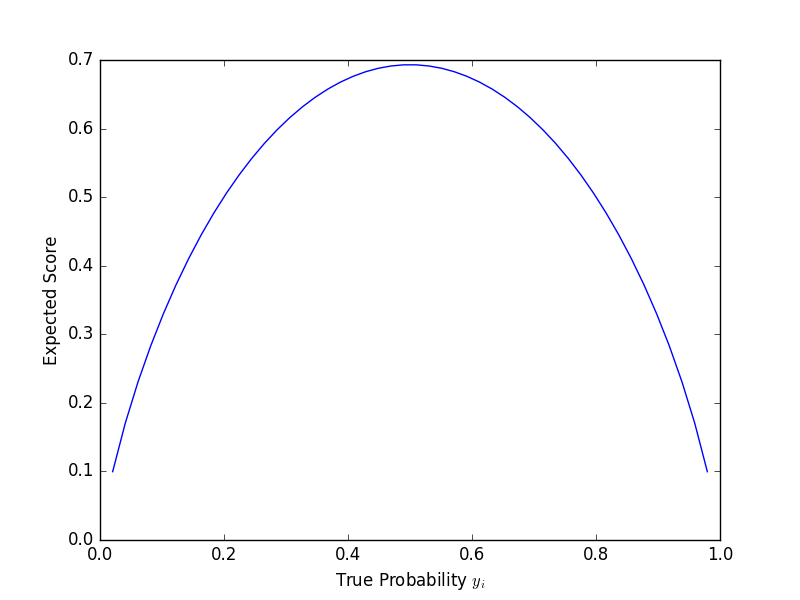
\includegraphics[scale=0.46]{expected_score}
\centering
\caption{Performance of a Perfect Knowledge Predictor}\label{Fig:perfm}
\end{figure}

\section{Data Sets}\label{Sec:data_set}
Kaggle provides almost three decades' data about NCAA basketball matches, including matches during the regular seasons as well as the tournaments. The data sets are summarised in Table~\ref{Ta:data_set}.
\begin{table}[h!]
\centering
\resizebox{\columnwidth}{!}{
\begin{tabular}{ | l | l | }
\hline
\textbf{Data Set} & \textbf{Description} \\ \hline
RegularSeasonCompactResults & Game-by-game results during regular seasons from 1985-2015\\ \hline
RegularSeasonDetailedResults & More detailed results during regular seasons from 2003-2015  \\ \hline
Seasons & Different seasons present in the dataset\\ \hline
Teams & Different college teams present in the dataset  \\ \hline
TourneyCompactResults & Game-by-game tournament results from 1985-2015 \\ \hline
TourneyDetailedResults & More detailed tournament results from 2003-2015.  \\ \hline
TourneySeeds & The seeds for all teams in a tournament  \\ \hline
TourneySlots & The pair-ups between two teams based on their seeds  \\ \hline
\end{tabular}}
\caption{A Summary of the Data Sets}\label{Ta:data_set}
\end{table}

However, not all data sets are useful. Only two of them are used in this project, namely \textbf{RegularSeasonCompactResults} and \textbf{Teams}. 

\section{Role Assignment}
Table~\ref{Ta:role_assgn} shows the assignment of roles for each team member in this project. 
\begin{table}[h!]
\centering
\resizebox{\columnwidth}{!}{
\begin{tabular}{ | l | l | l | }
\hline
\textbf{Team member} & \textbf{Role} & \textbf{Responsibility} \\ \hline
Joe Tan Chin Yong & Data Scientist & To build predictive models \\ \hline
Liu Zeyan & Data Analyst & To optimise selected models \\ \hline
Wei Yumou & Data Scientist & To build predictive models \\ \hline
Xie Dai & Statistician & To provide mathematical knowledge  \\ \hline
\end{tabular}}
\caption{Role Assignment}\label{Ta:role_assgn}
\end{table}


%2.0 DATASET
%
%We use three datasets in this project:
%
%2.1 RegularSeasonDetailedResults.csv
%
%This file identifies the game-by- game results for 13 seasons of historical data, from 2003 to 2015. Each year, it includes all games played from daynum 0 through 132.
%
%Each row in the file represents a single game played. It includes team-level total statistics for each game. We use the data from 2013 to 2015 as only the recent data is relevant to our prediction.

\chapter{Preliminary Analysis}\label{Chap:2}

\section{Challenges}

There are various challenges in tackling the problem, namely, which features to use, and which machine learning technique to use. There might also be a possible lack of direct match between two teams, where we will need to estimate the result.

%\subsection{Feature Selection}
%
%Features are pieces of information that may be useful for predictions. As mentioned in Section~\ref{Sec:data_set}, Kaggle provides a comprehensive set of various data which might be useful for us. However, we have to choose the features that satisfy the two criteria of usefulness and relevance to tackle this problem.

\subsection{Obsolete Data Sets}

Regardless of the machine-learning technique used, the most \emph{relevant} data is the historical match records during both regular and tournament seasons. However, some data sets contain match records that date back to as early as 1985, which are no longer \emph{useful} in today's context. After all, the NCAA tournament teams consist of \emph{college students} who can only stay with a team for a maximum of four years before graduation. Since only team-level data is available, it is difficult to quantify the effect that changes in a team's composition bring on the skill of that team, as players constantly leave and join the team. Moreover, there were some substantial updates on the Tournament's rules at the beginning of the 2008-2009 season~\cite{NP15}, which also affected the strategy teams used in the subsequent tournaments. Therefore, only the most recent match records are useful for prediction. For the purpose of this project, a four-year window from 2013 to 2016 is selected and all data used in this project fall within this window. 

\subsection{Complex Interrelationship}

No team is in isolation. The tournament matches are interactive processes whereby complex interrelationships exist amongst all the contesting teams, which adds another layer of complication in the attempt to predict match results. For example, given the history match records that Team A beaten Team B and Team C lost to Team B, one should intuitively conclude that Team A should have a higher probability of beating Team C. But what if another record shows that Team A once lost to Team C? In that case, the relative strength levels of the three teams will be hard to determine. Moreover, the match whose result is to be predicted may be the very \emph{first} match ever between two teams. In other words, there are no historical records that give a direct assessment on the two teams' strengths. Such lack of knowledge must be complemented by some interrelationships amongst the teams. So a good predictive model should not only be able to take into consideration the current game record, but also explore the interrelationships amongst all the game records and generalise on unseen matches. 

\subsection{The Curse of Model Popularity}


\chapter{TrueSkill\texttrademark~Rating System}\label{Chap:3}
TrueSkill~\cite{TS07} is a Gaussian rating system developed by Microsoft Research in 2007 to rank players on Xbox Live for the purpose of creating competitive matches for players with similar skill levels. While the Elo rating system is applicable to only two-player matches, the TrueSkill ranking system extends the use cases to multi-player matches. Section~\ref{Sec: tmm} discusses the Approximate Bayesian Inference --- the mathematical backbone of the TrueSkill rating system. Section~\ref{Sec: imp} presents the process of building predictive models based on an open-source implementation of the TrueSkill rating system. 

\section{Approximate Bayesian Inference}\label{Sec: tmm}

The approach described in Section~\ref{Sec: approach} can be modelled as a Bayesian Inference process. Define a vector $\matr{s}  = [s_{1}, s_{2}, \ldots, s_{n}]^{\intercal}$ representing the individual \emph{skill} of $n$ teams in a match (in the case of NCAA basketball tournament, $n = 2$). Further assume that each skill follows a Gaussian distribution $s_{i} \sim \mathcal{N}(\mu_{i}, \sigma_{i}^{2})$ and collectively, the \emph{prior} joint distribution of skills is a n-variate Gaussian distribution $p(\matr{s}) = \mathcal{N}_{n}(\matr{s}; \matr{\mu}, \matr{\Sigma})$

In a match, each team is expected to exhibit a certain \emph{performance} $p_{i} \sim \mathcal{N}(s_{i}, \beta_{i}^{2})$ that varies around its skill. The match result can be represented as a set of rankings in ascending order for each team, namely, $\matr{r} = [r_{1}, r_{2}, \ldots, r_{n}]^{\intercal}$ where $r_{1} \leq r_{2}, \ldots, r_{n - 1} \leq r_{n}$. In reality, there are many factors that may affect the outcome of a match, but for the purpose of Bayesian Inference, the assumption is that it is the differences in team performances that cause the differences in team rankings. According to the Bayes' Theorem, the posterior distribution $p(\matr{s} | \matr{r})$ is given by
\begin{equation}\label{Eqn: bayes}
p(\matr{s} | \matr{r}) = \frac{P(\matr{r} | \matr{s})p(\matr{s})}{P(\matr{r})} = \frac{P(\matr{r} | \matr{s})p(\matr{s})}{\int P(\matr{r} | \matr{s})p(\matr{s})d\matr{s}}
\end{equation}

The above formula demonstrates the use of Bayes' Theorem to calculate the updated skill distribution (posterior) given the match outcome (evidence) and the expectations (likelihood and prior) on the match outcome before the match. However, the posterior distribution is no longer a Gaussian distribution and oftentimes, the integral is intractable. A common solution is to calculate a Gaussian distribution $\mathcal{N}_{n}(\matr{s}; \hat{\matr{\mu}}, \hat{\matr{\Sigma}})$ as an approximation to the posterior distribution $p(\matr{s} | \matr{r})$ so that the Kullback-Leibler divergence between the two distributions is minimised. 

A number of approximation techniques are available. For the TrueSkill rating system, it approximates the posterior distribution by setting up a \emph{factor graph} which is a bipartite graph containing two kinds of vertices: variables and factors. A variable stores some value of interests and a factor represents some operations on one or more variables. The Bayesian Inference process is modelled as passing some \emph{message}s, which are some real-valued functions of a variable or a factor, throughout the factor graph. Figure~\ref{Fig:fact_grph} shows an example factor graph of a simple two-player match. Based on skill $s_{i}$ and performance $p_{i}$, it calculates the expected performance difference $p_{1} - p_{2}$ and compares that with an externally supplied outcome $d$. The $\mathbb{I}$ denotes an indicator function to assert whether $d$ is consistent with the expectation, depending on which a different update is performed on $s_{1}$ and $s_{2}$. 

\begin{figure}[h!]
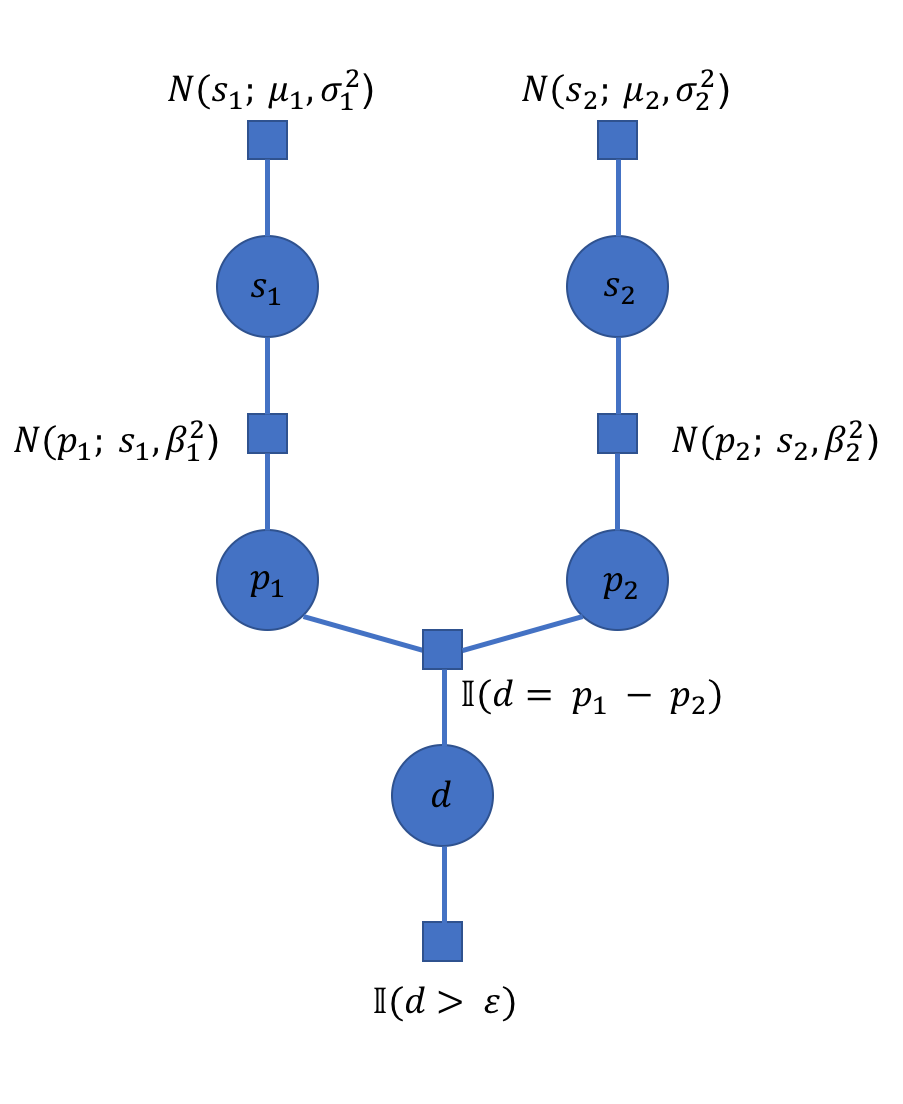
\includegraphics[scale=0.5]{factor_graph}
\centering
\caption{An example of factor graph}\label{Fig:fact_grph}
\end{figure}

The ultimate goal of a factor graph is to obtain a set of update equations that indicate how each $\mu_{i}$ and $\sigma_{i}$ should be updated. However, passing messages throughout larger factor graphs can involve very intensive computations. As suggested by~\cite{RC11}, there is an alternative but easier way of getting the same set of update equations based the following theorem. 
\begin{theorem}
Let $\matr{z}$ be a k-dimensional random vector $[z_{1}, z_{2}, \ldots, z_{k}]^{\intercal}$ with a probability distribution function of the form
\begin{equation}\label{Eqn: z_dist}
\frac{\phi_{k}(\matr{z})f(\matr{z})}{\int \phi_{k}(\matr{z})f(\matr{z})d\matr{z}}
\end{equation}
where $\phi_{k}$ is a k-variate standard Gaussian distribution function. Then, the expectation of $\matr{z}$ is given by
\begin{equation}
E[\matr{z}] = E\Big{[}\frac{\nabla f(\matr{z})}{f(\matr{z})}\Big{]}
\end{equation}
and also
\begin{equation}
E[z_{i}z_{j}] = \delta_{ij} + E\Big{[}\frac{\nabla^{2} f(\matr{z})}{f(\matr{z})}\Big{]}
\end{equation}
where $\delta_{ij} = 1$ if $i = j$ and $\delta_{ij} = 0$ otherwise. 
\end{theorem}

To link Equation~\ref{Eqn: z_dist} with the Bayes' Theorem in Equation~\ref{Eqn: bayes}, notice that the match outcome is dependent on performances and performances are related to skills; therefore, the likelihood probability $P(\matr{r} | \matr{s})$ can be expressed as some function of skill $f : \matr{s} \rightarrow [0, 1]$. Furthermore, since each $s_{i} \sim \mathcal{N}(\mu_{i}, \sigma_{i}^{2})$, define the z-score vector $\matr{z} = [z_{1}, z_{2}, \ldots, z_{n}]^{\intercal}$ where 
\begin{equation}
z_{i} = \frac{s_{i} - \mu_{i}}{\sigma_{i}} 
\end{equation}
Therefore, the probability distribution $p(\matr{z}) = \phi_{n}(\matr{z})$ and the likelihood probability $P(\matr{r} | \matr{s})$ is also a function of $\matr{z}$. Then according to Equation~\ref{Eqn: bayes}, 
\begin{equation}
p(\matr{z} | \matr{r}) = \frac{P(\matr{r} | \matr{z})p(\matr{z})}{P(\matr{r})} = \frac{\phi_{n}(\matr{z})f(\matr{z})}{\int \phi_{n}(\matr{z})f(\matr{z})d\matr{z}}
\end{equation}
The values of interest are $\matr{\mu}^{new}$ and $\matr{\Sigma}^{new}$, which is related to $E[\matr{z}]$ by
\begin{equation}
\matr{\mu}^{new} = E[\matr{s}] = E[\matr{\mu} + \matr{\Sigma}\matr{z}] = \matr{\mu} + \matr{\Sigma}E[\matr{z}]
\end{equation}
and
\begin{equation}
\matr{\Sigma}^{new} = Var[\matr{s}] = \matr{\Sigma}\matr{\Sigma}^{\intercal}Var[\matr{z}] = \matr{\Sigma}\matr{\Sigma}^{\intercal}E[(\matr{z} - E[\matr{z}])(\matr{z} - E[\matr{z}])^{\intercal}]
\end{equation}

\section{Implementation}\label{Sec: imp}
\chapter{Time-Dependent Edge Cost Estimation}\label{Chap:4}

%\chapter{Time-Dependent Shortest Path Calculation}\label{Chap:5}

%\chapter{Conclusion}\label{Chap:6}

%\appendix
%\chapter{Source Code}
\section{Database Utilities}
The source code listed in this section provides utility functions for general database operations, such as \textbf{select} and \textbf{update}. It is to be used in other modules. 

\begin{lstlisting}[language = PHP, caption = {Database Utilities}, label = {AList:db_utilities}, frame=single, numbers=left, stepnumber=1]
<?php
include "../inc/jingodbinfo.inc";

function connect_db(){
    $conn = new mysqli(DB_SERVER, DB_USERNAME, DB_PASSWORD);
    if($conn->connect_error){
	die("Connection failed: " . $conn->connect_error);
    }
    $conn->select_db(DB_DATABASE);
    $conn->set_charset("utf8");
    return $conn;
}

function disconnect_db($conn){ $conn->close(); }

function db_select($conn, $table, $cols, $cond = "true", $distinct = "")
{
    $sql_select = "SELECT {$distinct} ";
    if(count($cols) == 0){
        $sql_select .= "*,";
    }
    foreach ($cols as $col) {
        $sql_select .= "{$col},";
    }
    $sql_select = rtrim($sql_select, ",");
    $sql_select .= " FROM {$table} WHERE {$cond};";
    $ret = $conn->query($sql_select);
    $res = array();
    if($ret->num_rows > 0){
        while($row = $ret->fetch_assoc()){
            $curr = array();
            foreach ($cols as $col) {
                $curr[$col] = $row[$col];
            }
            $res[] = $curr;
	}
    }
    return $res;
}

function db_update($conn, $table, $values, $cond){
    $sql_update = "UPDATE {$table} SET ";
    foreach ($values as $key => $value) {
        if(is_numeric($value)){
            $sql_update .= "{$key} = {$value},";
        }else{
            $sql_update .= "{$key} = '{$value}',";
        }
    }
    $sql_update = rtrim($sql_update, ",");
    $sql_update .= " WHERE {$cond};";
    $succ = $conn->query($sql_update);
    return $succ;
}

function db_insert($conn, $table, $values, $cond = "", $ignore = ""){
    $sql_insert = "INSERT {$ignore} INTO {$table} ";
    $cols = "";
    $vals = "";
    foreach ($values as $key => $value) {
        $cols .= "{$key},";
        $vals .= (is_numeric($value) ? "{$value}," : "'{$value}',");
    }
    $cols = rtrim($cols, ",");
    $vals = rtrim($vals, ",");
    $sql_insert .= "({$cols}) VALUES ({$vals}) {$cond};";
    echo "{$sql_insert}\n";
    $conn->query($sql_insert);
}

function db_delete($conn, $table, $cond){
    $sql_delete = "DELETE FROM {$table} WHERE {$cond};";
}
?>
\end{lstlisting}

\clearpage
\newpage

\section{Data Pre-processing}
This section lists down the source code used in data pre-processing. 

\begin{lstlisting}[language = PHP, caption = {Outlier Removal}, label = {AList:outlier_rmvl}, frame=single, numbers=left, stepnumber=1]
<?php
include "db_utilities.php";

class Filter{
    private $ldmk_start;
    private $ldmk_end;
    private $ldmk_table;
    private $data_table;
    private $update_table;
    private $path;
    private $bchmk;
    
    private $conn;
    private $num_dele;
    
    public function __construct($ldmk_start, $ldmk_end, $ldmk_table, $data_table, $path, $bchmk, $update_table){
        $this->ldmk_start = $ldmk_start;
        $this->ldmk_end = $ldmk_end;
        $this->ldmk_table = $ldmk_table;
        $this->data_table = $data_table;
        $this->update_table = $update_table;
        $this->path = $path;
        $this->bchmk = $bchmk;
        $this->conn = connect_db();
        $this->num_dele = 0;
    }
    
    public function __destruct(){ disconnect_db($this->conn); }
    
    private function getCentres($ldmk){
        $filename = "{$this->path}{$ldmk}.csv";
        $centres = array();
        if(($handle = fopen($filename, 'r')) !== FALSE){
            while(($line = fgetcsv($handle, 0, ',')) !== FALSE){
                $centres[] = array($line[0], $line[1]);
            }
	}
	return $centres;
    }
    
    private function getRecords($ldmk){
        $ldmk_cols = array('LandmarkName');
        $ldmk_cond = "LandmarkID = {$ldmk}";
        $ret = db_select($this->conn, $this->ldmk_table, $ldmk_cols, $ldmk_cond);
        $data_cols = array('DataUnitID', 'BD09_LONG', 'BD09_LAT');
        $data_cond = "Street = '{$ret[0][$ldmk_cols[0]]}'";
        $ret = db_select($this->conn, $this->data_table, $data_cols, $data_cond);
        $records = array();
        foreach ($ret as $item) {
            $records[] = array($item[$data_cols[0]], $item[$data_cols[1]], $item[$data_cols[2]]);
        }
        return $records;
    }
    
    
    private function removeRecord($centres, $records){
        foreach ($records as $recd) {
            $min_dist = INF;
            foreach ($centres as $centre) {
                $min_dist = min($min_dist, $this->getHaversineDist
                ($centre[0], $centre[1], $recd[1], $recd[2]));
            }
            if($min_dist > $this->bchmk){
                $cond = "DataUnitID = {$recd[0]}";
                db_delete($this->conn, $this->data_table, $cond);
                ++$this->num_dele;
            }
	}
    }
    
    private function toRadian($degree){ return $degree * M_PI / 180; }
    
    private function getHaversineDist($long1, $lat1, $long2, $lat2){
        $BJ_LAT = $this->toRadian(39);
        $EQ_R = 6378137; // equatorial radius in metres
        $POL_R = 6356752; // polar radius in metres

	$BJ_R = sqrt((pow($EQ_R * $EQ_R * cos($BJ_LAT), 2) + pow($POL_R * $POL_R * sin($BJ_LAT), 2)) / (pow($EQ_R * cos($BJ_LAT), 2) + pow($EQ_R * sin($BJ_LAT), 2)));
	$long1 = $this->toRadian($long1);
	$lat1 = $this->toRadian($lat1);
	$long2 = $this->toRadian($long2);
	$lat2 = $this->toRadian($lat2);
	$d = 2 * $BJ_R * asin(sqrt(pow(sin(($lat1 - $lat2) / 2), 2) + 
	cos($lat1) * cos($lat2) * pow(sin(($long1 - $long2) / 2), 2)));
	return $d; }
    private function getWithin($ldmk, $centres, $records){
        foreach ($records as $recd) {
	    $min_dist = INF;
	    foreach ($centres as $centre) {
	        $min_dist = min($min_dist, 
		$this->getHaversineDist($centre[0], $centre[1], $recd[1], $recd[2]));
	    }
	    if($min_dist <= $this->bchmk){
	        db_insert($this->conn, $this->update_table, 
			array('LandmarkID' => $ldmk, 'BD09_LONG' => $recd[1], 'BD09_LAT' => $recd[2]));
	    }
	}
    }
    
    public function doFiltering(){
	for($ldmk = $this->ldmk_start; $ldmk != $this->ldmk_end; 
		++$ldmk){
	    $centres = $this->getCentres($ldmk);
	    $records = $this->getRecords($ldmk);
	    $this->getWithin($ldmk, $centres, $records);
	}
    }
}
set_time_limit(0);
ini_set('memory_limit','2048M');
$filter = new Filter($_POST['ldmk_start'], $_POST['ldmk_end'], 
	$_POST['ldmk_table'], $_POST['data_table'], $_POST['path'], 
	$_POST['bchmk'], $_POST['update_table']);
$filter->doFiltering();
?>
\end{lstlisting}

\section{Landmark Graph Construction}
This section presents algorithms related to landmark graph construction. 
\begin{lstlisting}[language = PHP, caption = {Trip Identification}, label = {AList:trip_identification}, frame=single, numbers=left, stepnumber=1]
<?php
include "db_utilities.php";

class IdentifyTrip{
    private $cuid_start;
    private $cuid_end;
    private $table;
    private $tripid;
    private $threshold;
    private $occup;
    private $conn;
    
    public function __construct($cuid_start, $cuid_end, $table, $tripid, $threshold, $occup){
    	$this->cuid_start = $cuid_start;
	$this->cuid_end = $cuid_end;
	$this->table = $table;
	$this->tripid = $tripid;
	$this->threshold = $threshold;
	$this->occup = $occup;
	$this->conn = connect_db();
    }
    
    public function __destruct(){ disconnect_db($this->conn); }



    public function startIdentifyTrip(){
    	$cols = array('DataUnitID', 'UnixEpoch');
	for($cuid = $this->cuid_start; $cuid != $this->cuid_end; 
		++$cuid){
	    $cond = "CUID = {$cuid} and Occupied = {$this->occup}";
	    $res = db_select($this->conn, $this->table, $cols, $cond);
	    if(count($res) > 0){
	        $this->splitTrip($res, $cols);
	    }
	}
    }
    
    public function splitTrip($res, $cols){
    	$last = $curr = $res[0][$cols[1]];
	foreach ($res as $item) {
	    $curr = $item[$cols[1]];
	    if($curr - $last > $this->threshold){
	    	++$this->tripid;
	    }
	    $values = array('TripID' => $this->tripid);
	    $cond = "{$cols[0]} = {$item[$cols[0]]}";
	    $succ = db_update($this->conn, $this->table, $values, 
	    	$cond);
	    $last = $curr;
	}
	++$this->tripid;
    }
}
set_time_limit(0); ini_set('memory_limit','2048M');
$identifyTrip = new IdentifyTrip($_POST['start'], $_POST['end'], $_POST['table'], $_POST['tripid'], $_POST['threshold'], $_POST['occup']);
$identifyTrip->startIdentifyTrip();?>
\end{lstlisting}

\begin{lstlisting}[language = PHP, caption = {Landmark Frequency}, label = {AList:ldmk_frequency}, frame=single, numbers=left, stepnumber=1]
<?php
include "db_utilities.php";
function insertLandmark($conn, $table, $landmark){
    $values = array("LandmarkName" => $landmark, "LandmarkCount" => 1);
    $cond = "ON DUPLICATE KEY UPDATE LandmarkCount = LandmarkCount + 1";
    $succ = db_insert($conn, $table, $values, $cond);
}
function fetchLandmark($conn, $table, $tripid){
    $cols = array("Street");
    $cond = "TripID = {$tripid} group by Street";
    $res = db_select($conn, $table, $cols, $cond);
    $streets = array();
    foreach ($res as $item) {
	foreach ($item as $key => $value) {
	    $streets[] = $value;
	}
    }
    return $streets;
}
set_time_limit(0); ini_set('memory_limit','2048M');
$conn = connect_db();
$start = $_POST['tripid_start']; $end = $_POST['tripid_end'];
$data_table = $_POST['dtable']; $landmark_table = $_POST['ltable'];
for($tripid = $start; $tripid != $end; ++$tripid){
    $landmarks = fetchLandmark($conn, $data_table, $tripid);
    foreach ($landmarks as $ldmk) {
  	$succ = insertLandmark($conn, $landmark_table, $ldmk);
    }
}
disconnect_db($conn);?>
\end{lstlisting}

\begin{lstlisting}[language = PHP, caption = {Landmark Construction}, label = {AList:ldmk_construction}, frame=single, numbers=left, stepnumber=1]
<?php
include "db_utilities.php";

class GraphBuilder{
    private $start;
    private $end;
    private $ldmktable;
    private $triptable;
    private $ldmklimit;
    private $holi_table;
    private $wrkd_table;
    private $conn;
    private $landmarks;

    public function __construct($start, $end, $ldmktable, $triptable, $ldmklimit, $holi_table, $wrkd_table){
	$this->start = $start;
	$this->end = $end;
	$this->ldmktable = $ldmktable;	
	$this->triptable = $triptable;
	$this->ldmklimit = $ldmklimit;
	$this->holi_table = $holi_table;
	$this->wrkd_table = $wrkd_table;
	$this->conn = connect_db();
	$this->landmarks = $this->fetchldmk();
    }

    public function __destruct(){ disconnect_db($this->conn); }



    private function fetchldmk(){
        $cols = array('LandmarkName', 'LandmarkID');
	$cond = "{$cols[1]} <= {$this->ldmklimit}";
	$res = db_select($this->conn, $this->ldmktable, $cols, $cond);
	$ldmks = array();
	foreach ($res as $item) {
	    $ldmks[$item[$cols[0]]] = $item[$cols[1]];
	}
	return $ldmks;
    }

    private function isLandmark($street){
	return array_key_exists($street, $this->landmarks);
    }

    private function isHoliday($atime){
	$date = date('d', $atime);
	$day = date('w', $atime);
	if($date == '01' || $date == '28' || $date == '29'){
	    return true;
	}else if($date == '31'){
	    return false;
	}else if($day == 0 || $day == 6){
	    return true;
	}
	return false;
    }





    public function buildGraph(){
	$street_cols = array("Street");
	$utc_cols = array("UnixEpoch");
		
	for($tripid = $this->start; $tripid != $this->end; ++$tripid){
	    $street_utc = array();
	    $street_cond = "TripID = {$tripid}";
	    $streets = db_select($this->conn, $this->triptable, $street_cols, $street_cond, "DISTINCT");
	    foreach ($streets as $item) {
		$street = $item[$street_cols[0]];
		$utc_cond = "{$street_cols[0]} = '{$street}' AND {$street_cond} LIMIT 1";
		$ret = db_select($this->conn, $this->triptable, $utc_cols, $utc_cond);
		if(count($ret) > 0){
		    $street_utc[$street] = $ret[0][$utc_cols[0]];
		}
	    }
	    $this->addEdge($street_utc, $tripid);
	 }
     }
     
    private function addEdge($street_utc, $tripid){
	$cols = array("LandmarkU", "Intermediate", "LandmarkV", "ArrivalTime", "LeavingTime", "Duration", "TripID");
	$streets = array_keys($street_utc);
	$size = count($streets);
	$low = 0;
	while($low < $size && !$this->isLandmark($streets[$low])){
	    ++$low;
	}
	$landmarkU = $landmarkV = $low < $size ? $streets[$low] : NULL;
	$atime = $ltime = $low < $size ? $street_utc[$landmarkV] : NULL;
	++$low;
	while($low < $size){
	    $inbetween = "";
	    while($low < $size && !$this->isLandmark($streets[$low])){
		$inbetween .= "{$streets[$low]}-";
		++$low;
	    }
	    $inbetween = rtrim($inbetween, "-");
	    $landmarkV = $low < $size ? $streets[$low] : NULL;
	    $ltime = $low < $size ? $street_utc[$landmarkV] : NULL;
	    if(!is_null($landmarkU) && !is_null($landmarkV)){
		$vals = array($landmarkU, $inbetween, $landmarkV, $atime, $ltime, $ltime - $atime, $tripid);
		if($this->isHoliday($atime)){
		    db_insert($this->conn, $this->holi_table, array_combine($cols, $vals));
		}else{
		    db_insert($this->conn, $this->wrkd_table, array_combine($cols, $vals));
		}
	     }
	     $landmarkU = $landmarkV;
	     $atime = $ltime;
	     ++$low;
	}
    }
}

set_time_limit(0);
ini_set('memory_limit','2048M');
date_default_timezone_set("Asia/Singapore");

$graphBuilder = new GraphBuilder($_POST['tripid_start'], $_POST['tripid_end'], $_POST['ldmktable'], $_POST['triptable'], $_POST['ldmklimit'], $_POST['holi_table'], $_POST['wrkd_table']);

$graphBuilder->buildGraph();
?>
\end{lstlisting}
%\chapter{Figures}

\vspace*{-3in}

\begin{figure}
\vspace{2.4in}
\caption{Armadillo slaying lawyer.}
\label{arm:fig1}
\end{figure}
\clearpage
\newpage

\begin{figure}
\vspace{2.4in}
\caption{Armadillo eradicating national debt.}
\label{arm:fig2}
\end{figure}
\clearpage
\newpage

%\bibliography{main}
%\bibliographystyle{alpha}
%% This defines the bibliography file (main.bib) and the bibliography style.
%% If you want to create a bibliography file by hand, change the contents of
%% this file to a `thebibliography' environment.  For more information 
%% see section 4.3 of the LaTeX manual.
\begin{singlespace}
%\bibliographystyle{IEEEtran}
%\bibliography{IEEEabrv,mybibfile}
\bibliography{main}
\bibliographystyle{amsplain}
\end{singlespace}

\end{document}

